%% the Hole argument 

%%

\documentclass[fleqn]{beamer}
\usetheme{metropolis}
\usepackage[utf8]{inputenc}
\usepackage[T1]{fontenc}
\usepackage{amsmath, amssymb}
\usepackage{graphicx}
\usepackage{hyperref}
\usepackage{amsfonts}
\usepackage{tikz-cd}


\usepackage{tikz}
\usetikzlibrary{decorations.pathreplacing, arrows.meta, positioning}

\usepackage{minted}
\usemintedstyle{tango} 

\title{Defining Determinism}
\subtitle{}
\author{Hans Halvorson}
\institute{Princeton University}
\date{April 11, 2025}

\usepackage[style=authoryear, backend=biber, natbib=true, doi=true]{biblatex} % Chicago style with Biber backend
\addbibresource{~/research/determinism/det.bib}

\begin{document}

\begin{frame}
  \titlepage
\end{frame}

\section{Introduction}

\begin{frame}{Introduction}

  %% You've got no choice!

  {\Huge
    Who cares about determinism? }


\end{frame}

\begin{frame}{The hole argument}

  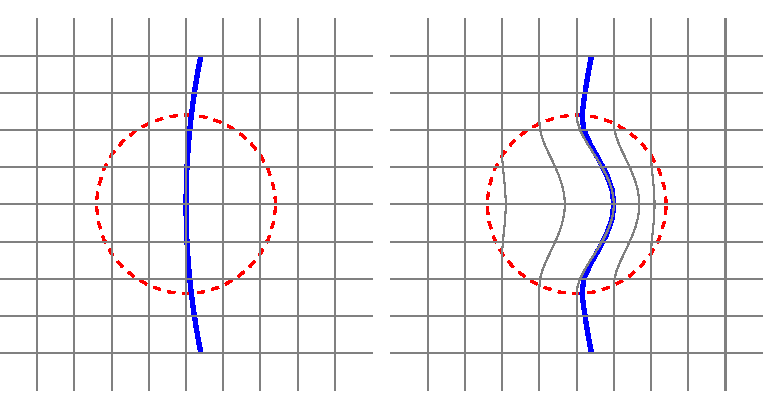
\includegraphics[scale=0.8]{hole.pdf}

%% but wait: what is determinism? Is this a failure of determinism?  

\end{frame}

\begin{frame}[fragile]{Deformation Function $\varphi$}
\begin{minted}[fontsize=\small]{haskell}
-- Deformation phi: identity on boundary, max push at center,
-- horizontal only
phi :: Double -> P2 Double -> P2 Double
phi r p@(P (V2 x y))
  | dist >= r  = p
  | otherwise  = p .+^ r2 (0.5 * bump, 0)  -- push right only
  where
    v     = p .-. origin
    dist  = norm v
    t     = dist / r
    bump  = (1 - t^2)^2  -- max at center, 0 at edge
\end{minted}
\end{frame}


\begin{frame}{Logical Structure of the Hole Argument}

\centering
\scalebox{0.6}{%
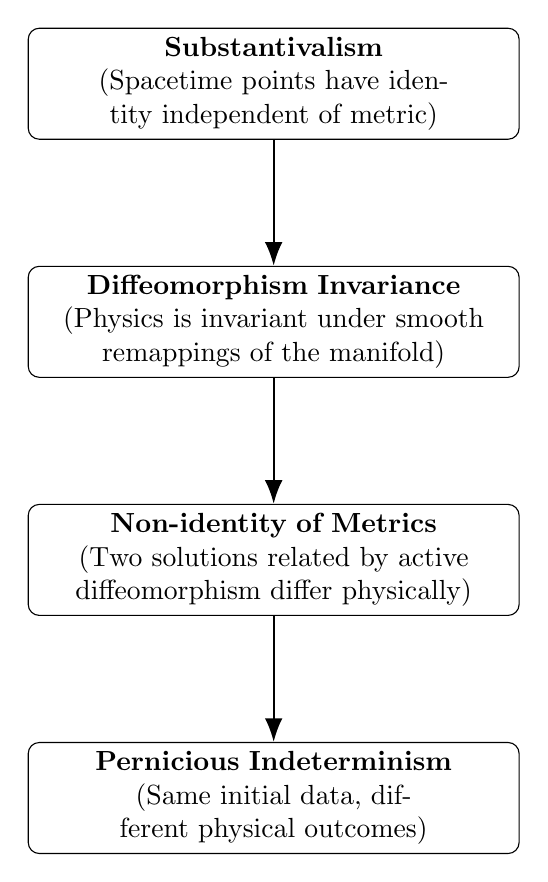
\begin{tikzpicture}[
    node distance=1.6cm and 2cm,
    every node/.style={font=\normalsize},
    box/.style={rectangle, draw, rounded corners, text width=6cm, align=center, minimum height=1cm},
    arrow/.style={-{Latex[length=3mm]}, thick}
  ]

  \node[box] (sub) {\textbf{Substantivalism}\\
  (Spacetime points have identity independent of metric)};
  
  \node[box, below=of sub] (diff) {\textbf{Diffeomorphism Invariance}\\
  (Physics is invariant under smooth remappings of the manifold)};
  
  \node[box, below=of diff] (nonid) {\textbf{Non-identity of Metrics}\\
  (Two solutions related by active diffeomorphism differ physically)};
  
  \node[box, below=of nonid] (indet) {\textbf{Pernicious Indeterminism}\\
  (Same initial data, different physical outcomes)};
  
  \draw[arrow] (sub) -- (diff);
  \draw[arrow] (diff) -- (nonid);
  \draw[arrow] (nonid) -- (indet);

\end{tikzpicture}
}


\end{frame}


\begin{frame}{Outline}
  \tableofcontents
\end{frame}

\section{Detour through theories?}

\begin{frame}{Carnap}

  ``The opposition between the determinism of classical physics and
  the probability determination of quantum physics concerns a
  syntactical difference in the system of natural laws, that is, of
  the P-rules of the physical language.'' \citep[p 307]{lsl}

\end{frame}

\begin{frame}{Carnap}

  \begin{description}
  \item[Metaphysical] Every process is univocally determined by its
    causes.
  \item[Syntactic] For every particular physical sentence $\varphi$,
    there is for any time coordinate $t$, which has a smaller value
    than the time coordinate which occurs in $\varphi$, a class
    $\Gamma$ of particular sentences with $t$ as time coordinate, such
    that $\varphi$ is a P-consequence of $\Gamma$. \end{description}


  \end{frame}

\begin{frame}{J.J.C. Smart}

  ``A perfectly precise meaning can be given to saying that certain
  theories are deterministic or indeterministic (for example that
  Newtonian mechanics is deterministic, quantum mechanics
  indeterministic), but our talk about actual events in the world as
  being determined or otherwise may be little more than a reflection
  of our faith in prevailing types of physical theory.'' \citep[p
  294]{smart-free}

\end{frame}

\begin{frame}{The end of an era}

  ``Many philosophical discussions of determinism are couched in terms
  of theories, construed as linguistic entities. But since determinism
  is a doctrine about the nature of the world, no problem is avoided
  by this linguistic detour.'' \citep[20]{primer}


\end{frame}

\begin{frame}{The end of an era}

  ``In the philosophical literature, there are two common criteria for
  a physical theory to be deterministic. The older one is due to the
  logical empiricists, and is a purely formal criterion. The newer one
  can be found in the work of John Earman and David Lewis and depends
  on the intended interpretation of the theory. In this paper I argue
  that the former must be rejected, and something like the latter
  adopted.'' (Belot 1995, p 85)

\end{frame}  

\section{The era of Lewis}

\begin{frame}{Lewis}

  A system of laws of nature is Deterministic iff no two divergent
  worlds both conform perfectly to the laws of that system. Second, a
  world is Deterministic iff its laws comprise a Deterministic
  system. Third, Determinism is the thesis that our world is
  Deterministic. \citep[p 360]{lewis-work}


\end{frame}

\begin{frame}{Lewis}

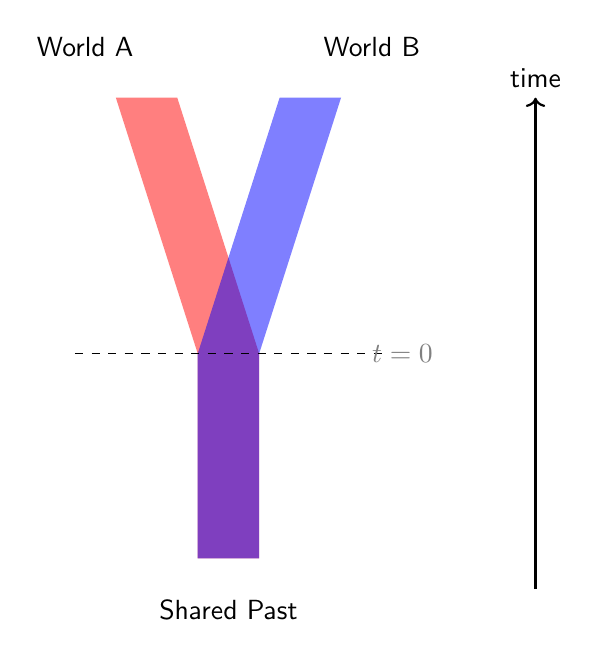
\begin{tikzpicture}[scale=1.3]

  % Tube half-width
  \def\tube{0.3}
  \def\bottom{-2}
  \def\split{0}
  \def\top{2.5}
  \def\dx{0.8}

  % === Red tube: vertical below t=0, tips left above
  \fill[red, opacity=0.5]
    (-\tube,\bottom) --
    (-\tube,\split) --
    (-\tube - \dx,\top) --
    (\tube - \dx,\top) --
    (\tube,\split) --
    (\tube,\bottom) -- cycle;

  % === Blue tube: vertical below t=0, tips right above
  \fill[blue, opacity=0.5]
    (-\tube,\bottom) --
    (-\tube,\split) --
    (-\tube + \dx,\top) --
    (\tube + \dx,\top) --
    (\tube,\split) --
    (\tube,\bottom) -- cycle;

  % Time axis
  \draw[->, thick] (3,\bottom - 0.3) -- (3,\top ) node[above] {\textsf{time}};

  % Dashed line at t = 0
  \draw[dashed] (-1.5,\split) -- (1.5,\split);
  \node[gray] at (1.7,\split) {$t=0$};

  % Labels
  \node at (-\dx - 0.6,\top + 0.5) {\textsf{World A}};
  \node at (\dx + 0.6,\top + 0.5) {\textsf{World B}};
  \node at (0,\bottom - 0.5) {\textsf{Shared Past}};

\end{tikzpicture}


\end{frame}

%% the ambiguity in Lewis

\begin{frame}{Determinism De Re}

  \emph{Qualitative Determinism:} For all times $t$, there is no
  possible world which matches this world in its qualitative
  description up to $t$, and which has the same laws of nature as this
  world, but which doesn't match this world in its total qualitative
  description. \citep[239]{hawthorne}

  \bigskip \emph{De Re Determinism:} For all times $t$, there is no
  possible world which matches this world in its de re description up
  to $t$, and which has the same laws of nature as this world, but
  which doesn't match this world in its total de re
  description. \citep[239]{hawthorne}


\end{frame}

\begin{frame}

\noindent \begin{figure}[h]
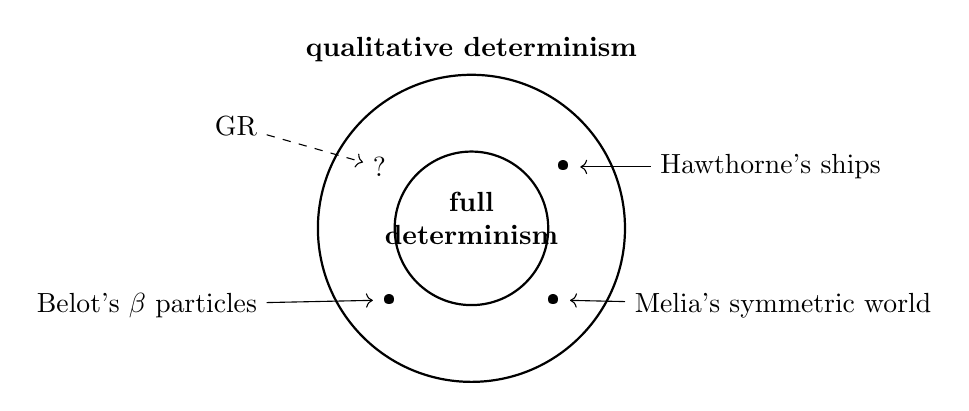
\begin{tikzpicture}[scale=0.65]
    % Draw the outer circle (Qualitative Determinism)
    \draw[thick] (0,0) circle (3cm);
    \node at (0,3.5) {\textbf{qualitative determinism}};

    % Draw the inner circle (De Re Determinism)
    \draw[thick] (0,0) circle (1.5cm);
    \node[align=center] at (0,0.2) {\textbf{full} \\ \textbf{determinism}};

    % Define positions for the black dots
    \node (GR) at (-1.8,1.2) {?};
    \node (Ships) at (1.8,1.2) {\textbullet};
    \node (Belot) at (-1.6,-1.4) {\textbullet};
    \node (Melia) at (1.6,-1.4) {\textbullet};

    % Place labels outside the outer circle with arrows pointing to dots
    \node[left] (GR_label) at (-4,2) {GR};
    \draw[->, dashed] (GR_label) -- (GR);

    \node[right] (Ships_label) at (3.5,1.2) {Hawthorne's ships};
    \draw[->] (Ships_label) -- (Ships);

    \node[left] (Belot_label) at (-4,-1.5) {Belot's $\beta$ particles};
    \draw[->] (Belot_label) -- (Belot);

    \node[right] (Melia_label) at (3,-1.5) {Melia's symmetric world};
    \draw[->] (Melia_label) -- (Melia);

  \end{tikzpicture}
  \label{fig2}
  \caption{Theories that are supposed to be qualitatively, but not
    fully, deterministic.}
\end{figure}

\end{frame}

\section{Formal conditions}

\begin{frame}{Semantics done right}

  \begin{itemize}
  \item Lewis' talk of possible worlds is verbal metaphor that finds
    its best explication in logical semantics
  \item When a vague metaphor is supposed to answer precise questions
    (e.g.\ is General Relativity deterministic), it gives funny
    answers.
    \begin{itemize}
    \item Theoretical equivalence: how do judge that two families of
      models say the same thing?
    \end{itemize}
  \item Don't forget the arrows!   
  \end{itemize}

  
\nocite{melia}
\end{frame}



\begin{frame}{Triple B}

  \textbf{D1.} A world $W$ is deterministic if, whenever $W'$ is
  physically possible with respect to $W$ and $t,t'$, and
  $f:W_t\to W_{t'}$ are such that $f$ is a duplication, there is some
  duplication $g:W\to W'$.

\end{frame}

\begin{frame}{Triple B}

  \textbf{D2.}  $W$ is deterministic if, whenever $W'$ is physically
  possible with respect to $W$, and $t,t'$, and $f:W_t\to W'_{t'}$ are
  such that $f$ is a duplication, there is some duplication
  $g:W\to W'$ whose restriction to $W_t$ is $f$.

\end{frame}

\begin{frame}{Triple B}

  \textbf{D3.} A world $W$ is deterministic if, whenever $W'$ is physically
  possible with respect to $W$, and $t,t',W'$ and $f:W_t\to W'_{t'}$
  are such that $f$ is duplication, then there is exactly one
  duplication $g:W\to W'$ which extends~$f$. \citep{belot}


\end{frame}

\begin{frame}[fragile]{The one true definition of determinism}

\begin{columns}[c]  % [c] for vertical centering

  \column{0.4\textwidth}
  {\Large
  \[
  \begin{tikzcd}
    M \arrow[r, "g", dashed] & M' \\
    U \arrow[u, hookrightarrow, "i"] \arrow[r, "f"'] & U' \arrow[u,
    hookrightarrow, "i'"']
  \end{tikzcd}
  \]
  }

  \column{0.6\textwidth}
  \begin{itemize}
  \item $U \hookrightarrow M$ is an embedding of an initial segment.
  \item For each isomorphism $f:U\to U'$ of initial segments, there is
    a unique isomorphism $g:M\to M'$ of worlds.
  \item Determinism: data on $U$ determines behavior in $M$.
  \end{itemize}

\end{columns}





\end{frame}

\begin{frame}

  \noindent \begin{figure}[h]
  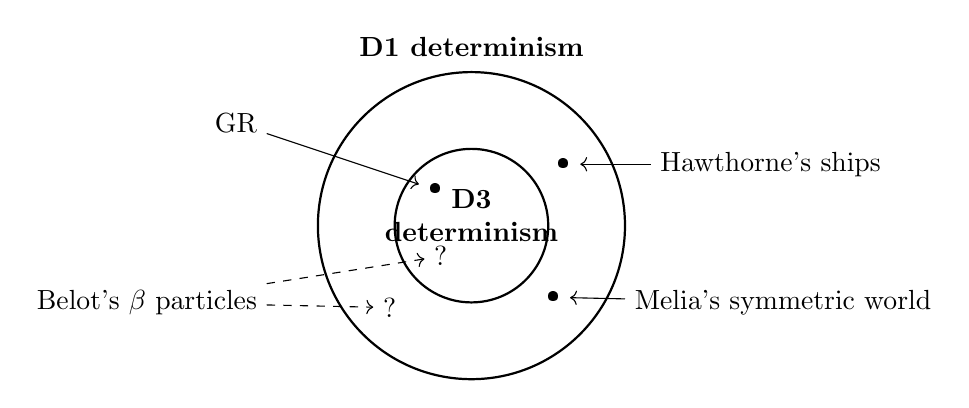
\begin{tikzpicture}[scale=0.65]
    % Draw the outer circle (Qualitative Determinism)
    \draw[thick] (0,0) circle (3cm);
    \node at (0,3.5) {\textbf{D1 determinism}};

    % Draw the inner circle (De Re Determinism)
    \draw[thick] (0,0) circle (1.5cm);
    \node[align=center] at (0,0.2) {\textbf{D3} \\ \textbf{determinism}};

    % Define positions for the black dots
    \node (GR) at (-0.7,0.7) {\textbullet};
    \node (Ships) at (1.8,1.2) {\textbullet};
    \node (Belot) at (-1.6,-1.6) {?};
    \node (Alt) at (-0.6,-0.6) {?};
    \node (Melia) at (1.6,-1.4) {\textbullet};

    % Place labels outside the outer circle with arrows pointing to dots
    \node[left] (GR_label) at (-4,2) {GR};
    \draw[->] (GR_label) -- (GR);

    \node[right] (Ships_label) at (3.5,1.2) {Hawthorne's ships};
    \draw[->] (Ships_label) -- (Ships);

    \node[left] (Belot_label) at (-4,-1.5) {Belot's $\beta$ particles};
    \draw[->, dashed] (Belot_label) -- (Belot);
    \draw[->, dashed] (Belot_label) -- (Alt);

    \node[right] (Melia_label) at (3,-1.5) {Melia's symmetric world};
    \draw[->] (Melia_label) -- (Melia);

  \end{tikzpicture}
  \caption{The toy examples in the literature are D3-indeterministic,
    while GR is D3-deterministic. Belot's example can be interpreted
    in two ways, one deterministic and one indeterministic.}
\end{figure}

\end{frame}

\section{Conclusion}

\begin{frame}{Lessons}

  \begin{itemize}
  \item All this business about ``property of theories versus
    ontological thesis'' is a distraction.
  \item Possible worlds talk is great \dots until we start making it
    really precise, and then it creates its own problems.
  \item Hawthorne's distinction between de re and de dicto determinism
    is non-natural.
  \item My proposal:
    \begin{enumerate}
    \item Remember that models of a theory form a \textbf{category},
      so that determinism depends on the arrows.
    \item Adopt Belot's D3 definition of determinism.
    \end{enumerate}
  \end{itemize}

\end{frame}




\section{References}

\begin{frame}[allowframebreaks]{References}

\printbibliography[heading=none]

\end{frame}


\begin{frame}{Belot's decay model}
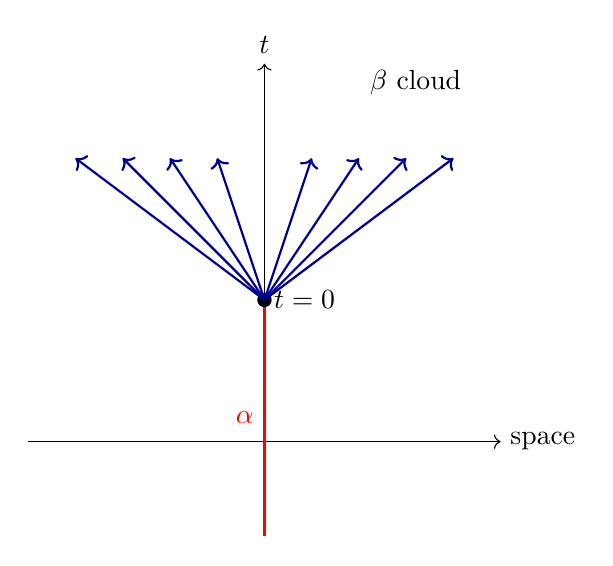
\begin{tikzpicture}[scale=1.2]
  % Axes
  \draw[->] (0,0) -- (0,4) node[above] {$t$}; % time axis
  \draw[->] (-2.5,0) -- (2.5,0) node[right] {space};

  % Alpha trajectory
\draw[red, line width=1.2pt] (0,-1) -- (0,1.5) node[pos=0.5,left] {$\alpha$};

  % Decay point
  \filldraw[black] (0,1.5) circle (2pt) node[right] {$t=0$};

  % Beta rays: same vertical height (e.g. t = 4), varying horizontal displacement
\foreach \x in {-2.0, -1.5, -1.0, -0.5, 0.5, 1.0, 1.5, 2.0} {
  \draw[thick, ->, blue!60!black] (0,1.5) -- (\x,3);
}

  % Label for beta cloud
  \node at (1.6,3.8) {$\beta$ cloud};

\end{tikzpicture}

\end{frame}







\end{document}

%%% Local Variables:
%%% mode: latex
%%% TeX-master: t
%%% End:
